\documentclass[11pt,a4paper]{article}
\usepackage[utf8]{inputenc}
\usepackage{amsmath}
\usepackage{amsfonts}
\usepackage{amssymb}
\usepackage{amsthm}
\usepackage{tikz}
\usepackage{graphicx}
\usepackage{algorithm}
\usepackage{algorithmic}

\usepackage[left=2cm,right=2cm,top=2cm,bottom=2cm]{geometry}
\author{Paul LANDRIER}
\title{Abstraction of computation graphs}

\newcommand{\bb}[1]{\mathbb{#1}}
\newcommand{\mcal}[1]{\mathcal{#1}}
\newcommand{\N}{\bb{N}}
\newcommand{\R}{\bb{N}}
\newcommand{\Cinf}{\mcal{C}^\infty}
\newcommand{\Ns}{near-semiring}

\date{}

\usetikzlibrary{shapes}

\newtheorem{theorem}{Theorem}

\newtheorem{definition}{Definition}
\newtheorem{ns}{Near-semiring}

\begin{document}

\maketitle

\section{Introduction}

We try to abstract the notion of \textit{computation graphs}, having in mind the particular example of neural networks.

	Computation graphs are a type of graphs that represent a computation. Formally, in this work, we define a computation graph $(V,E,Fun,Op)$ as a directed acyclic graph $(V,E)$ together with a function $Fun:E \to F$ where $F$ is a set of functions $S \to S$ ($S$ is a fixed set, the same for all functions) and a function $Op:V \to Operator$ where $Operator$ is a set containing operators to aggregate several inputs in $S$. (Remark : usually in a computation graph, the functions are stored in the nodes and the edges represent a data dependency. We choose a different convention here to remain closer to provenance in graphs).
	
	For instance, if we want to compute the function $f(x)=e^{x^2}(x^2 + 2x + 2)$ using only the linear, "plus constant" and exponential functions, with $+$ and $\times$ operators, then we can model a possible computation with the computation graph :
	
	\begin{figure}[!h]
	\centering
	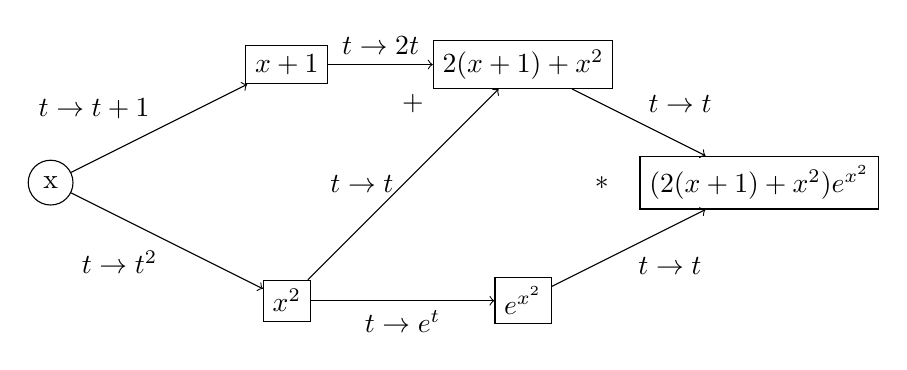
\begin{tikzpicture}
	
		\node[circle,draw] (x) at (0,0) {x};
		\node[rectangle,draw] (a) at (3,1.5) {$x+1$};
		\node[rectangle,draw] (b) at (3,-1.5) {$x^2$};
		\node[rectangle,draw] (c) at (6,1.5) {$2(x+1) + x^2$};
		\node at (4.6,1) {$+$};
		\node[rectangle,draw] (d) at (6,-1.5) {$e^{x^2}$};
		\node[rectangle,draw] (e) at (9,0) {$(2(x+1) + x^2)e^{x^2}$};
		\node at (7,0) {$*$};
		
				\path[->] (x) edge node[midway,above left] 
			{$t \to t+1$} (a);
		\path[->] (x) edge node[midway,below left]
			{$t \to t^2$} (b);
		\path[->] (a) edge node[midway,above] 
			{$t \to 2t$} (c);
			
		\path[->] (b) edge node[midway,left] 
			{$t \to t$} (c);
		\path[->] (b) edge node[midway,below] 
			{$t \to e^t$} (d);
		\path[->] (c) edge node[midway,above right]
			{$t \to t$} (e);
		\path[->] (d) edge node[midway,below right] 
			{$t \to t$} (e);
		
	\end{tikzpicture}
	\caption{One possible computation graph of $f$.}
	\label{fig:graphe_calc_ex}
	\end{figure}
	
	Let's take the example of a (non-discretized) perceptron with two inputs. If we want to model its execution using only elementary operations and the activation function $f$, we get :
	
	\begin{figure}[!h]
\label{fig:graph_calc_execution}
\centering
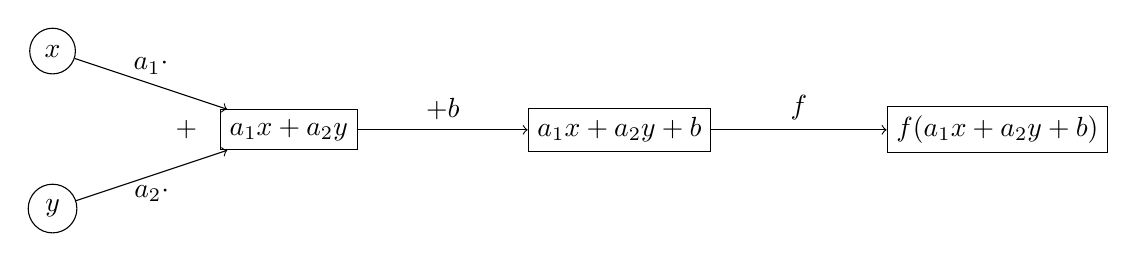
\begin{tikzpicture}

	\def\layersep{3cm}	
	
	\node[circle,draw] (x) at (0,1) {$x$};
	\node[circle,draw] (y) at (0,-1) {$y$};
	\node[rectangle,draw] (a) at (\layersep,0) {$a_1 x + a_2 y$};
	\node (plus) at (\layersep - 1.3cm,0) {+};
	\node[rectangle,draw] (c) at (2.4*\layersep,0) {$a_1 x + a_2 y + b$};
	\node[rectangle,draw] (e) at (4*\layersep,0) {$f(a_1 x + a_2 y + b)$};
	
	\path[->] (x) edge node[midway,above] {$a_1 \cdot $} (a);
	\path[->] (y) edge node[midway, below] {$a_2 \cdot$} (a);
	
	\path[->] (a) edge node[midway,above] {$ + b$} (c);
	
	\path[->] (c) edge node[midway,above] {$f$} (e);
	
	
\end{tikzpicture}
\caption{Computation graph of a perceptron.}
\end{figure}


\section{Executing a computation}

\subsection{Model}

We attempt to characterize the minimal algebraic structure required to model a computation graph. We fix $S$ the domain of the functions and, keeping in mind our targeted use case, we assume that there is only one operator : $Operator = \{ + \}$.
\\

The full computation represented by the graph cannot be expressed in a similar fashion as for provenance in graphs ($\underset{\pi \in P_{x,y}}{\sum} w(\pi)$) because composition does not distribute over $+$. In a general computation graph, the algorithm to execute the computation consists of executing the nodes following a topological ordering (by executing a node we mean executing all the functions that enters the node, sum their result and store the value).

Another way to see it is to define the input as the nodes in the graph with in-degree 0 and the output as the node in the graph with out-degree 0. The algorithm to retrieve the function represented by the computation graph from the definition is then a recursive algorithm that builds the function starting at an output node with function identity.
\\

\begin{algorithm}
\caption{Retrieve Function}
\label{alg:retrieve_function}
\begin{algorithmic}[1]
\STATE \textbf{Function} RetrieveFunction(Graph)
\STATE \hspace{1em} Output $\leftarrow$ Graph.Output
\STATE \hspace{1em} Result $\leftarrow$ Retrieve(Output, IdentityFunction)
\STATE \hspace{1em} \textbf{Return} Result
\STATE \textbf{End Function}
\end{algorithmic}
\end{algorithm}

\begin{algorithm}
\caption{Retrieve}
\label{alg:retrieve}
\begin{algorithmic}[1]
\STATE \textbf{Function} Retrieve(Node, F)
\STATE \hspace{1em} \textbf{If} Node.IsInput \textbf{Then}
\STATE \hspace{2em} \textbf{Return} F
\STATE \hspace{1em} \textbf{Else}
\STATE \hspace{2em} Result $\leftarrow$ ZeroFunction
\STATE \hspace{2em} \textbf{For Each} (Ancestor, G, Node) \textbf{In} Node.IncomingEdges \textbf{Do}
\STATE \hspace{3em} Result $\leftarrow$ Result + Retrieve(Ancestor, Compose(F, G))
\STATE \hspace{2em} \textbf{End For}
\STATE \hspace{2em} \textbf{Return} Result
\STATE \hspace{1em} \textbf{End If}
\STATE \textbf{End Function}
\end{algorithmic}
\end{algorithm}

\begin{figure}[!h]
	\centering
	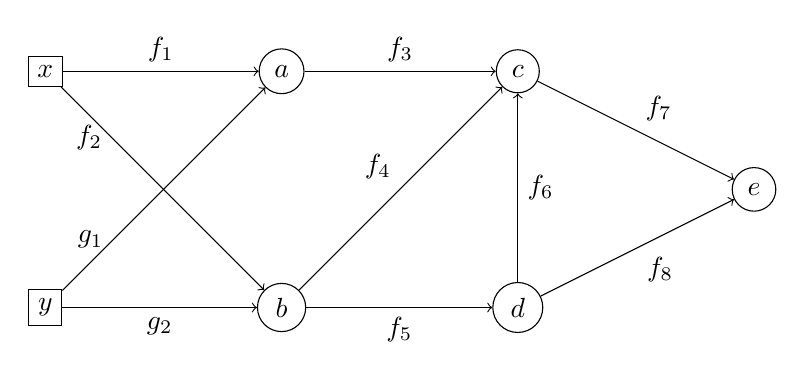
\begin{tikzpicture}
	
		\node[rectangle,draw] (x) at (0,1.5) {$x$};
		\node[rectangle,draw] (y) at (0,-1.5) {$y$};
		\node[circle,draw] (a) at (3,1.5) {$a$};
		\node[circle,draw] (b) at (3,-1.5) {$b$};
		\node[circle,draw] (c) at (6,1.5) {$c$};
		\node[circle,draw] (d) at (6,-1.5) {$d$};
		\node[circle,draw] (e) at (9,0) {$e$};
		
		\path[->] (x) edge node[midway,above] 
			{$f_1$} (a);
		\path[->] (x) edge node[near start, left=0cm]
			{$f_2$} (b);
		\path[->] (y) edge node[near start, left=0cm] 
			{$g_1$} (a);
		\path[->] (y) edge node[midway,below]
			{$g_2$} (b);
		\path[->] (a) edge node[midway,above] 
			{$f_3$} (c);
			
		\path[->] (b) edge node[midway,above left] 
			{$f_4$} (c);
		\path[->] (b) edge node[midway,below] 
			{$f_5$} (d);
		\path[->] (d) edge node [midway,right] 
			{$f_6$}(c);
		\path[->] (c) edge node[midway,above right]
			{$f_7$} (e);
		\path[->] (d) edge node[midway,below right] 
			{$f_8$} (e);
		
	\end{tikzpicture}
	\caption{An abstract computation graph.}
	\label{fig:graphe_calc_abstr}
	\end{figure}

\paragraph{Structure needed} We consider a structure $(F,\circ,+,0,id)$. The $+$ and $\circ$ are operators $F^2 \to F$ respectively used to model aggregation and composition in the computation graph.

Following what has been made in \textit{provenance semirings} by Green, Karvounarakis and Tannen and by Ramusat in its thesis, in order to identify the structure that best fits our application we try to identify some remarkable properties of computation graph to deduce some properties on the structure used to generalize them. We sum up the process in the table:

\begin{tabular}{|c|c|}
\hline 
\textbf{Property on the coputation graph} & \textbf{Algebraic Traduction of the property} \\ 
\hline 
The edges that enter a node are not ordered & + is associative and commutative \\ 
The concatenation of two computation graphs is a computation graph that represent the composition of the functions & $\circ$ is associative \\ 
\hline 
• & • \\ 
\hline 
• & • \\ 
\hline 
• & • \\ 
\hline 
\end{tabular} 

Since there is no natural order on incoming edges for a node, $+$ must be associative and commutative so the sum on incoming edges is well-defined. (For instance consider the node $c$ in Figure \ref{fig:graphe_calc_abstr}).

We require the operator $\circ$ to be associative so that computations in the graph can proceed either from left to right or from right to left to retrieve the function it represents, and to ensure modularity, which allows us to define the function associated with a subgraph.

To abstract the concept of zero-weight, we require the existence of a neutral element $0$ which is a left absorbing element for the $\circ$ operator and which is a neutral element for $+$.

We require the left distributivity $(f+g) \circ h = f \circ h + g \circ h$ beacuse it is of theoretical interest (it is necessary for the interpretation of near-semirings as sub-near-semirings of the the complete near-semiring over a monoid), because it is a natural identity to interpret the elements as functions and because it allows for a simplification of the computation in some cases.

Finally, we require the existence of a neutral element $id$ for $\circ$. This might not be crucial and could change, but it has interexting theoretical properties (it allows to model the one node graph for instance, which can be useful to initialize some algorithms such as Retrieve earlier). 
\\

The axiom identified are those of a near-semiring, with two differences (+ is not assumed to be commutative in general and the "id" does not necessarily exist). In our case, we obtain the definition:

\begin{definition}[Near-semiring]

	A \textit{near-semiring} $(F,+,\circ,0_F,id)$ is a set $F$ equiped with two binary operations $+,\circ$ and two distinguished elements $0_F,id$ such that :
	
	\begin{itemize}
	
		\item $(F,+,0_F)$ is a commutative monoid;
		
		\item $(F,\circ,id)$ is a monoid;
		
		\item $\forall (f,g,h) \in F^3$, $(f+g) \circ h = f \circ h + g \circ h$;
		
		\item $0_F$ is left absorbing for $\circ$, i.e. for all $f \in F$, $0_F \circ f = 0_F$.
			
	\end{itemize}

\end{definition}

Together with this definition comes the notion of morphism of near-semiring and of sub-near-semiring:

A sub-near-semiring of a near-semiring $(F,+,\circ,0,id)$ is a subset $G \subset F$ such that $0 \in G, id \in G$ and $G$ is stable by $+$ and $\circ$. If $G$ is a sub-near-semiring of $(F,+,\circ,0,id)$, then $(G,+,\circ,0,id)$ (for the restriction of operations + and $\circ$ to $G$) forms a near-semiring.

If $(F,+,\circ,0,id)$ and $(G,+',\circ ',0',id')$ are two near-semirings, then $\phi : F \to G$ is said to be a near-semiring morphism if it satisfies $\phi(0)=0',\phi(id)=id',\forall (f,g) \in F^2, \phi(f+g) = \phi(f) +' \phi(g)$ and $ \phi(f \circ g)= \phi(f) \circ' \phi(g)$.

\subsection{Examples}

We should now study a few examples of near-semiring.

\begin{ns}[Near-semiring over a monoid]
\label{ns:ns_over_a_monoid}
	Let $(M,+,0_M)$ be a monoid. We define $\mcal{F}$ the set of all functions $M \to M$. Then the tuple $(\mcal{F},+,\circ,0_F,id)$ where $0_F : x \mapsto 0_M$ is the zero function and $id : x \mapsto x$ is the identity function is a near-semiring, that we will call complete \Ns\ over $M$. A particular sub-\Ns\ of $\mcal{F}$ is the set of monoid endomorphisms of $M$.
\end{ns}

\begin{ns}[Semirings]
\label{ns:semirings}
	Let $(S,+,\cdot,0,1)$ be a semiring. Then $(S,+,\cdot,0,1)$ is also a \Ns . Indeed, the axioms of \Ns\ are stricly more general than those of a semiring. The interpretation of semirings as sets of function together with the interpretation of $\cdot$ as a composition can be made through the structure of semimodules, which is itself a sub-\Ns\ of the complete \Ns\ over a monoid.
\end{ns}

\subsection{Universal object}

The \Ns\ generated by a finite number of elements.

\subsection{Generality of the complete semiring over a monoid.}

\begin{theorem}{Universal Form of Near-semirings}

	It is equivalent to be given:
	
	\begin{enumerate}
	
		\item a near-semiring $(F,+,\circ,0,id)$
		
		\item a monoid $(M,+,0)$ together with a set of functions $M \to M$ containing $0$ and $id$ and stable by $\circ$ and $+$.
	
	\end{enumerate}

\end{theorem}

\begin{proof}

	Firstly, we assume that we are given a monoid $(M,+,0)$ and a set of functions $M \to M$ containing $0$, $id$ and stable by $+$ and $\circ$ like in two. This means that we are given a sub

\end{proof}

\section{Training a model}

Want to add a derivative $d$. Forces to add a $\cdot$. What identities ? $\to$ $d(f \circ g)$ ?

\section{Experiments ?}

\end{document}